\documentclass{article}
\usepackage{blindtext}
\usepackage[utf8]{inputenc}
\usepackage{graphicx}
\usepackage{amsmath, amsfonts}
\usepackage{float}
\usepackage[section]{placeins}
\usepackage{fancyvrb}
\usepackage[affil-it]{authblk} 
\usepackage{verbatim}

\pagenumbering{arabic}
\title{Math 381: Discrete Mathematical Modeling Project 2}
\author{Yanni Du, Tim Turner, Yuqi Huang, Evan Ko }
\affil{University of Washington}
\date{August 16 2017}
\begin{document}
	
\maketitle
\newpage
\tableofcontents
\newpage

\section{Abstract}

What would you do if you knew Apple's price per share in the stock market 30 days from now? \\
Buying or selling shares based on the net change is probably at the top of your list!
Over the course of the paper, we examine the process for modeling stock, analyze the types of events that effect stock price, and try to predict the future price per share of a stock. \\
In constructing our model and analyzing events, we use Apple as an example for applying the ideas we develop. \\
Through testing our model using Monte Carlo simulation, we find interesting results and discuss the sensitivity of our analysis. \\
\text{[Compress last couple of lines above.]} \\
\text{[Add few sentences summarizing results / findings.]} \\

\section{Problem Description}
\subsection{Problem}

Predict price per share of a stock (e.g. Apple) 30 days from day of latest known price with historical data.\\

\subsection{Background}
Inherently, stock prices are \textit{not} known in advance or predictable with complete certainty, simply because any number of events can occur that might effect the price of a stock. The Random Walk Theory even suggests that stock price changes have the same distribution and are independent of each other, so the past movement or trend of a stock price or market cannot be used to predict its future movement.\cite{RW}\\
However, in the real world, this theory is never popular among investigators, especially when people have fast access to relevant news and resources nowadays. Even in cases where our prediction might not be accurate, we hope there will be precision in our results evidenced through proportional effect caused by different events.

\subsection{Questions}

Some questions we're looking to answer include
\begin{itemize}
	\item What equations provide the best elements for a model and why?
    \item What things affect stock? Events, stock age, company, time of day, etc
    \item What events might affect a stock?
    \item Which types of events are more likely to affect a stock?
    \item Can events be profiled with properties that show the magnitude of their impact on a stock?
    \item Do similar event profiles share similar probability distributions?
    \item How do multiple factors, each with their own unique effect, combine to affect stock?
\end{itemize}

\section{Simplifications and Modeling}
\subsection{Simplification and Assumptions}
In this project, we simplify the Brownian model of financial markets. The model has some original assumptions that we are also using: \cite{WikiBModel}
\begin{itemize}
	\item We assume a frictionless market that no transaction costs occur either for buying or selling.
    \item The asset has continuous prices evolving in time and are driven by Geometric Brownian motion processes.
    \item There are no surprises in the market. 
\end{itemize}
In our project, instead of analyzing the price of a portfolio, which is the combination of investing in bond and stocks, we simplify the model by only analyzing one stock price, the stock price of Apple. We also add one more assumption that the stock does not pay a dividend.\\
With these simplifications, we are now focusing our project on a part of an investment instead of the whole portfolio. We still give a nice model showing how Monte Carlo simulation is used in finance. \\
Additionally, we are going to simulate the stock price based on Geometric Brownian Motion in this project instead of Brownian motion, which is used in the original model. Brownian motion is a continuous-time stochastic process. However, since Brownian motion takes negative values, it is questionable to model the stock price. On contrary, Geometric Brownian Motion is the exponential of the Brownian Motion process, one of the reasons that geometric Brownian motion is used to model financial and other processes that cannot be negative.\cite{GBMoverBM} \\

\section{Mathematical Model}

\subsection{Model Adaptation for Monte Carlo}
In order to convert our simplified model into a mathematical model that can be solved using a Monte Carlo simulation we need to find or choose what values will be used for our parameters and how we will implement our randomness in the random variable component.\\
To this end, in our specific case we have for any given day $t \in \{1,2,...,30\}$ the next day's predicted stock price $S_{t+1}$ will close according to:

\begin{align*}
S_{t+1} = S_{t}exp\left [ \left ( \mu -\frac{\sigma ^{2}}{2} \right ) +\sigma \epsilon \right ] \\
\end{align*}

Constant Drift component: $\mu - \frac{\sigma ^{2}}{2}$
\begin{itemize}
\item Historical Average Return ($\mu$)  - Average rate of return over historical
\item Historical Variance ($\sigma^{2}$) - Variance over historical data
\end{itemize}

Random Shock component: $\sigma \epsilon$
\begin{itemize}
\item Historical Standard Deviation ($\sigma$) - Standard deviation over historical data.
\item Z-Score of Random Number ($\epsilon$) - Z-Score for normal distributed mean zero random number with standard deviation of one.
\end{itemize}

Thus we arrive at the mathematical model for simulation, described as:
\begin{align*}
S_{t+1} &= S_{t}exp( \text{drift} + \text{shock} ) \\
&= S_{t}exp \left [ \left ( \text{Mean} - \frac{\text{Var}}{2} \right ) + \text{StdDev} * \text{Z-Score(Rand[0,1])} \right ]
\end{align*}

To transform the mathematical model for Monte Carlo simulation:\\
- Use random number between zero and one for random element in our random variable.\\
- Consider the resulting random number to be a percent, and calculate resulting

\subsection{Analysis of Random Variables, Parameters}
- Drift:\\
a) Historical Average\\
b) Variance component\\
- Shock:\\
a) Standard deviation component\\
b) Random Z-score from random number.\\
- Geometric using exponential function\\

\noindent\textbf{Parameters:}\\
Drift:
\begin{itemize}
\item Historical Average ($\mu$) is a constant value, taken as the mean of the rates of return for each day in the interval from August 11, 2016 to August 11, 2017. This is the average rate of return for Apple's stock over the course of the last 12 months.
\item Historical Variance ($\sigma ^{2}$) is a constant value, taken as the square of the standard deviation for the same historical interval of the previous 12 months.
\end{itemize}
Shock:
\begin{itemize}
\item Historical Standard Deviation ($\sigma$) is a constant value, taken as the standard deviation for the same interval of 12 months.\\
\end{itemize}

\noindent\textbf{Random Variables:}\\
\begin{itemize}
\item Randomized Z-Score ($\epsilon$) is the z-score for a randomly distributed mean zero random variable, with standard deviation of one.
\end{itemize}

\subsection{Alternative Modeling Strategies}
- Adding additional parameters to add information to the system from existing data. \\
- Adding additional random variables results in more complex, but possibly more naive or inconsistent model.

We found a more complex strategy was used in a recent study that contributed additional informative parameters to the drift which helped describe a given stock's behavior in the market. The capital pricing asset model (CAPM) augments the $\mu$ component of the drift with additional parameters:
\begin{align*}
\mu = r_{f} + \beta_{m}(r_{m} - r_{f})
\end{align*}

\noindent These parameters provide additional information:
\begin{itemize}
\item Risk-free Rate of Return ($r_{f}$) is an alternate form of expected return not derived directly from a stock's historical behavior, but instead guaranteed (risk-free) by the stock. An example of this rate might be a savings account at a bank that always provides a risk-free return for money stored in that account.
\item Beta Against Market ($\beta_{m}$) is the 
\item Expected Return of Market Portfolio ($r_{m}$) is 
\end{itemize}

\noindent\text{[Integrate quote as citation for different strategies]}
"Sengupta (2004) state that there are numerous measures of the expected rate of return that can be used for the model, such as the expected rate based on historical returns and estimates from analysts. Abidin and Jaffar (2014) used the mean percentage change in stock prices over one month because they were looking at forecasting stock prices from an investor’s perspective, rather than from a corporate finance standpoint." [1](pg. 28-29)

\subsection{Benefits of Chosen Strategy}
- Relatively accurate most of the time, negative return (loss) is unlikely.\\
- Tangible numbers for probability of best, worst, avg cases happening for risk mitigation.

\section{Solution of the Mathematical Model}

\subsection{Algorithm Description}

\text{[Basically discuss the variables and loop(s) from the code, and how they relate to the math model]}\\
Explanation of our algorithm:
\begin{enumerate}
\item To begin, we read in the data from the csv file
\item Then we calculate the mean, variance, and standard deviation of the previous year's return data
\item we predict numPred days of closing price data using our algorithm. Our algorithm uses a shock and drift factor to estimate the future stock price.
\begin{itemize}
\item  The drift factor is calculated by the mean of the return - (variance/2) ($drift = \mu - \frac{\sigma^2}{2}$)
\item The shock factor is calculated by taking the product of the standard deviation of the return and the z-score of a random number generated between 0 and 1 ($shock = \sigma*(z-score(rand[0-1]))$
\end{itemize}
\item To estimate the future price we take the product of the previous day's closing price and the result of the e raised to the power of the sum of the drift and shock. ($S_{t+1} = S_t*e^{drift + shock}$)
\item To get a more accurate prediction we run the simulation nTrial times. A higher number of runs trends the data towards a a normal distribution
\item to analyze the predicted data for the 30th day we calculate the mean, varience, and standard deviation of all the trial's 30th day prediction.
\item we then estimate the 
\end{enumerate}
\text We generated our own algorithm to generate future stock prices. Using mathematical formulas that we found in some of the literature, we altered the formulas to best fit our model. 

\subsection{Algorithm Solution}
Our model:\\
\begin{verbatim}
###############################
#Code for modeling a Monte Carlo Stock Price Problem

#Variables
#S = Today's Price
#TP = Tomorrow's Price
#meanR = mean of the rate of return
#varR = varience of the rate of return
#sdR = standard Deviation of the rate of return

#Equations used
#TP = S*e^r
#x = Random number between 0 and 1
#r = (u-sig^2/2) + (sdr)* (Z-score(x)
###############################
#import data from the excel file
library(RCurl)

url <- "https://raw.githubusercontent.com/evanzko/Math-381-Final-Project/master/AAPL-1year-basic.csv"
#download data
data <- getURL(url) 
#read data from csv file
MyData <- read.csv(text = data)


#calculate statistical variables from the return calculated from 2016-2017
meanR <- mean(MyData[,'Return'], na.rm = TRUE) 
varR <- var(MyData[,'Return'], na.rm = TRUE)
sdR <- sd(MyData[,'Return'], na.rm = TRUE)

#parameters for model
drift <- meanR - (varR/2)
thisYr <- MyData[,'Close'] #real data from 2016-2017 
numPred <- 30 #the number of days the model is predicting
nTrials <- 1000 #the number of trials the model is running

#create a matrix for multiple trials. Each column represents one trial. Each row is a day
A = matrix(numeric(nTrials*numPred), nrow = numPred, ncol = nTrials, byrow = TRUE)
#set the initial prediction value of the matrix as the last value of the closing price
A[1,] = thisYr[length(MyData$Close)]

#make a prediction for the next year
for(i in 1:nTrials){
  for(j in 2:numPred){
    rand <- runif(1, 0.0, 1.0) #choose a random number between 0-1
    S <- A[j-1,i] #get the last closing price
    shock <- sdR*qnorm(rand) #standard deviation*z-score
    delta <- exp(drift + shock) #calulate the change factor of the stock
    A[j,i] <- S*delta #predict the closing price of the jth day
  }
}

#Statistical analysis of predicted price
Price30 <- A[numPred,]
meanP30 <- mean(Price30)
varP30 <- var(Price30)
sdP30 <- sd(Price30)
#95% CI
error <- qnorm(0.975)*sdP30/sqrt(nTrials)
left <- meanP30 - error
right <- meanP30 + error




\end{verbatim}
\section{Results}

\subsection{Statistical Analysis of the Result}
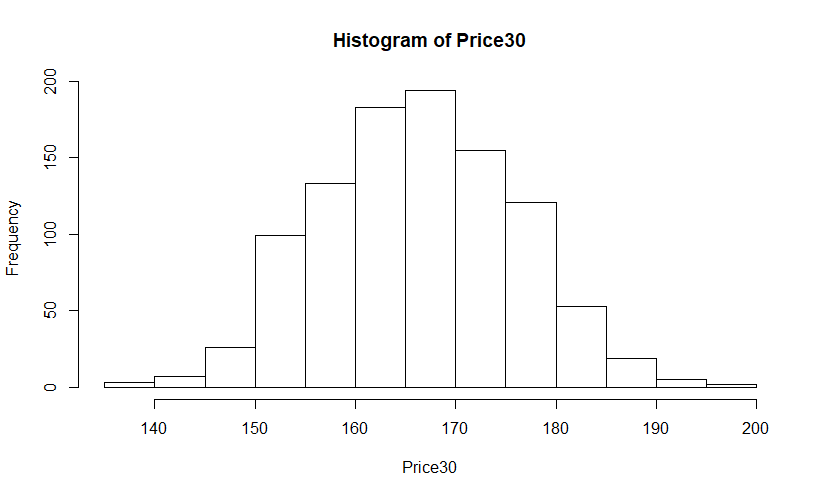
\includegraphics[width = \textwidth]{Rplot.png}
The table below shows the mean, variance, standard deviation, standard error and 95\% confidence interval of the stock price of Apple in 30 days:
\begin{table}[hbt]
  \centering
  \caption{Statistical Analysis}
  \label{stat}
  \begin{tabular}{|l|l|l|l|l|l|l|}
  \hline
  \multicolumn{1}{|c|}{} & Mean   & Variance & SD & SE & 95\% CI Lower & 95\% CI Upper \\ \hline
  Stock Price in 30 days & 166.31 & 94.41    & 9.72               & 0.60           & 165.71              & 166.91              \\ \hline
  \end{tabular}
\end{table}

\subsection{Risks}
We are at risk of:\\
a) the final price not being what was expected after a given interval of time,\\
b) an unlikely high or repeated shock due to non-historical events.\\
c) Since we did not constantly update the drift in this model, $S_t$ will go to infinity as $t \rightarrow \infty$ with probability 1.\cite{GBM}

\subsection{Reasonableness}
Our result is reasonable as long as our assumption is solid, that there are no surprises in the market. For example, a new employment policy or a new product would dramatically drive up the stock price.  Meanwhile, the human behavior is also hard to model. In the real stock market, the stock price changes because of people buying in and selling out. When a big investment company tries to buy in or sell out some stock, this behavior can be infectious and may cause big changes to the price. Additionally, people often expect the stock price to drop after a period time of increasing and even there is no sign in the market, people will start selling out because they are afraid of the ``upcoming drop”. 


\subsection{Validation}

\subsection{(\textasciitilde) Baseline Comparison}

\section{Conclusions}

For baseline comparison we decided it would be most telling to try and compare our model to real data, the historical change in stock price over the previous year.\\
We use the year before that to get our historical average and then try to predict a year's worth of price changes. Then compare the results to what really happened after that year.\\
In doing this we found a wide range, plus or minus forty dollars, in predicted final stock price vs actual stock price. However, there is a normal distribution showing that most of the time the resulting stock price was within a difference of just ten dollars.


\pagebreak
\begin{thebibliography}{9}
\bibitem{ApplicationGBM}
Simulating Stock Prices Using Geometric Brownian Motion: Evidence from Australian
Companies
\bibitem{WikiBModel}
Wikipedia: Brownian Model of Financial Markets\\
\texttt{https://en.wikipedia.org/wiki/Brownian-model-of-financial-markets}
\bibitem{RW}
http://www.investopedia.com/terms/r/randomwalktheory.asp
\bibitem{WikiBSModel}
Wikipedia: Black-Scholes Model\\
\texttt{https://en.wikipedia.org/wiki/Black-Scholes-model\# Short-stock-rate}
\bibitem{GBMoverBM}
http://www.columbia.edu/\~ ks20/FE-Notes/4700-07-Notes-GBM.pdf
\bibitem{GBM}
http://www.math.uah.edu/stat/brown/Geometric.html
\end{thebibliography}


\begin{itemize}
	\item https://sites.math.washington.edu/~billey/classes/math.480.spring.2016/course.notes/381notes.pdf
    \item http://www.maths.manchester.ac.uk/~pjohnson/resources/math60082/lecture-monte-carlo-ls.pdf
	\item http://www.investopedia.com/articles/07/montecarlo.asp
	\item https://www.youtube.com/watch?v=3gcLRU24-w0
	\item https://www.mathworks.com/discovery/monte-carlo-simulation.html
    
\end{itemize}

	
	
	
\end{document}
